\section{Research questions, concepts and propositions}
\label{sec:question}
\subsection{Interlocking directorates}
Companies are embedded in complex networks of `interlocking directorates' -- 
created when directors from a corporation sit on multiple boards.
The relationship between two corporations resulting from a director sitting in both of their boards is often referred to as a direct interlock~\citep{Mizruchi1996}.
Interlocks can also be indirect when two directors from two firms sit together on the board of directors of a third firm. 
Several explanations (micro-motives) have been pointed out for the creation of interlocks. 
These include facilitating cooperation to limit competition (collusion),  
absorption of potentially disruptive elements (cooptation), 
creating legitimacy by hiring respectable directors, 
career advancement, and social cohesion~\citep{Mizruchi1996}.

Although the micro-motives for the existence of interlocks are relatively well understood, 
their effects are still object to controversy. 
In the past decades, many papers have investigated the effect of interlocks in firm performance [ref], innovation [ref], acquisitions [ref], mergers [ref], capital growth [ref], firm reputation [ref], and adoption of structures and strategies [ref]. See Mizruchi~\cite{Mizruchi1996} for a review.
However, only the spread of structures and strategies has been consistently associated to interlocks [refs].
We attribute this to limitations in data analysis.
Previous papers have focused on a small number of top companies (10--1000), 
many times restricting the study to only one sector or country. 
The result of this approach is a misrepresentation of local patterns as global patterns.
For example, 
[this example with this data, ref] found that the presence of interlocks increases firm growth.
At the same time,
[this example with this other data, ref] found that the presence of interlocks decreases firm performance.


% simple explanation by Mizruchi~\cite{Mizruchi1996} that 
%For instance,  points out that if directors are appointed when the productivity of the firm is low (as a form of monitoring),
%and directors decide to join boards that are performing well (as a form of career development),
%the end result would be an inverted U shaped relationship between number of interlocks and firm performance. 
%This model would explain why researchers [refs] have found positive and negative relationship between interlocks and performance,


We study a large dataset comprising 200 million companies and 100 million directors (see \ref{sec:data}) to bring definitive answers to the field .
Our main research question is ``How is the network of interlocking directorates structured in time and space, and what is its effect on structural transformation?''.
For the sake of brevity, we focus here on the second part of the question ``what is the effect of interlocks on structural transformation'',
where structural transformation corresponds to the evolution of the distribution of economic activities within the city.
In section \ref{sec:pss} we explore the concepts of structural transformation and the product-service space.
The product-service space determines how closely two economic activities (sectors) are depending on how many cities have companies in both sectors.
In section \ref{sec:interlockspss}, we determine if (and how) interlocks affect structural transformation.
Section \ref{sec:factors} shows what factors influence the presence of interlocks.
Our unit of analysis can be the company itself, the city, the country or the region. 
For clarity, 
because cities have became innovation hubs~\citep{Belderbos2014}, 
and because we should not impose a national structure on interlock data~\citep{Heemskerk2016},
we will focus on the city level for the rest of the manuscript.


\subsection{Product-service space}
\label{sec:pss}
Cities and countries develop economically by moving from producing simple products and services to specializing in more expensive ones -- a process referred to as `structural transformation'~\citep{smith1776, Romer1991,grossman1991,hidalgo2007}.
This transformation can be explained using differences in productive factors and technology (see~\citep{hausmann2011} for a review).
In order to connect these differences to development, 
current models usually abstract from the products and look at macro-indicators of productive factors and technology.
However, development occurs when new products are created or existing ones improved,
and it is not clear if these models can explain the variability observed in countries with similar macro-indicators.
Moreover, the products that are developed depend on the current products being produced -- there is a relatedness between products.
Many explanation have been proposed for this, 
such as similar institutions, infrastructure, physical factors, technology, or some combination of those factors (see~\cite{hidalgo2007} for a review).
Hidalgo, Hausman and Klinger~\cite{hidalgo2007, hausmann2011, Hausmann2006,hidalgo2009} assume that related products require similar underlying factors (`capabilities'),
and developed the `product space' as a map of the relatedness between products,
where products are related if countries have competitive advantages respect to both products.
They showed that the product space capture information about the set of capabilities available in a country, 
is strongly correlated with income per capita, 
and predictive of future growth.
Furthermore, they proved that structural transformation at the country level occurs by moving from existing products to related products, 
where two products are related if they are closed in the `product space'.

In a world full of multi-nationals, innovation is happening at the city level~\citep{Belderbos2014}.
To account for a fine-grained exploration of the process, we adapt the `product-space' concept. 
We focus on relationships between economic activities at the city level,
instead of product categories at the country level.
Using cities allows us to explore not only products, but also services, thus we will define the `product-service space'. 
The subquestion here is: ``Does structural transformation at the city follows the links of the product-service space''.
We expect to find comparable trends at the city level than Hidalgo, Hausman and Klinger found at the country level.
The structural transformation should follow the edges in the product-service space, 
and the diffusion process should correlate with gdp per capita in the city, 
and maybe with innovation, for which we can use the city Innovation index \footnote{\url{http://www.innovation-cities.com/innovation-cities-index-2015-global/9609}}
or the number of patents developed in companies from the city.
The causal argument is symmetrical from Hidalgo, Hausman and Klinger's argument~\cite{hidalgo2007, hausmann2011, Hausmann2006,hidalgo2009} but at the city level.
Cities require some underlying capabilities (infrastructure, education, institutions, human capital) to maintain specific companies,
and those capabilities are similar for economic activities close together in the product-service space.
When a city acquire new capabilities, new products can be developed along the product-service space.
Since we are more interesting in understanding the role of interlocks in the process, 
the aim of this section is descriptive, 
but hinting on causality.
Negative results would suggest an extreme globalization of the cities, 
where the benefit of having `in situ' capabilities is minimal.


%We will define the network as $PSS = (V, E)) $, where $V$ are the sectors according to NACE rev. 2 (e.g. C11 = Manufacture of beverages),
%and $E$ is the matrix of weights between sectors.


\subsection{Interlocks and the PSS}
\label{sec:interlockspss}
%[Research subquestion herere]
Next, we will analyze if interlocks are a good predictor of diffusion between economic activities in cities. 
Development itself influences the presence of interlocks.
Companies situated close geographically, or in places with similar language or colonial ties 
have greater chances to interlock [refs].
Since the establishment of companies in the city allow for greater possibilities of interlocks,
we expect a relationship between the product-service space and the number of interlocks between economic activities.
However it is not clear if interlocks are only a cause of development but also an effect.
Interlocks provide a communication channel between companies, 
and serve as a link for the spread of strategies and structures (refs).
For instance, [examples of previous research].
We hypothesize that interlocks serve as a communication channel for opportunities,
thus increasing investment and R\&D to sectors close in the product-service space.
The increased investment and innovation has been linked to development~\citep{Romer1991,grossman1991,hidalgo2007}.
In a first step, we will test if interlocks affect the diffusion process in the product-service space.
In a second step, we will analyze collaboration between companies using patent data to show if this diffusion process is mediated (at least partially) by innovation.

\subsubsection{Interlocks affect the PSS}
%[Research subquestion herere]
Figure ~\ref{fig:entropy} shows our approach. 
Given the number of companies in city A at time t (Fig. ~\ref{fig:entropy}A), 
we want to explain the evolution to time t+1 (Fig. ~\ref{fig:entropy}B).
Hidalgo and Hausmann~\cite{hidalgo2009} showed that this evolution (at the country level) is related to the `product space' (Fig. ~\ref{fig:entropy}C).
We can create a network of interlocks (Fig. ~\ref{fig:entropy}D),
where two economic activities are connected if a director sits in companies from both sectors.
Importantly, the network of interlocks have relationships between sectors that are not present in Figure ~\ref{fig:entropy}A. 
This is because interlocks are not restricted to the city itself.
A director can sit in the banking sector in city A and in the IT sector in city B, even if there are no IT companies in city A.
Our research question here is then ``To what extent do interlocks increase the diffusion rates in the product-service space?''.


\begin{figure}
\begin{center}
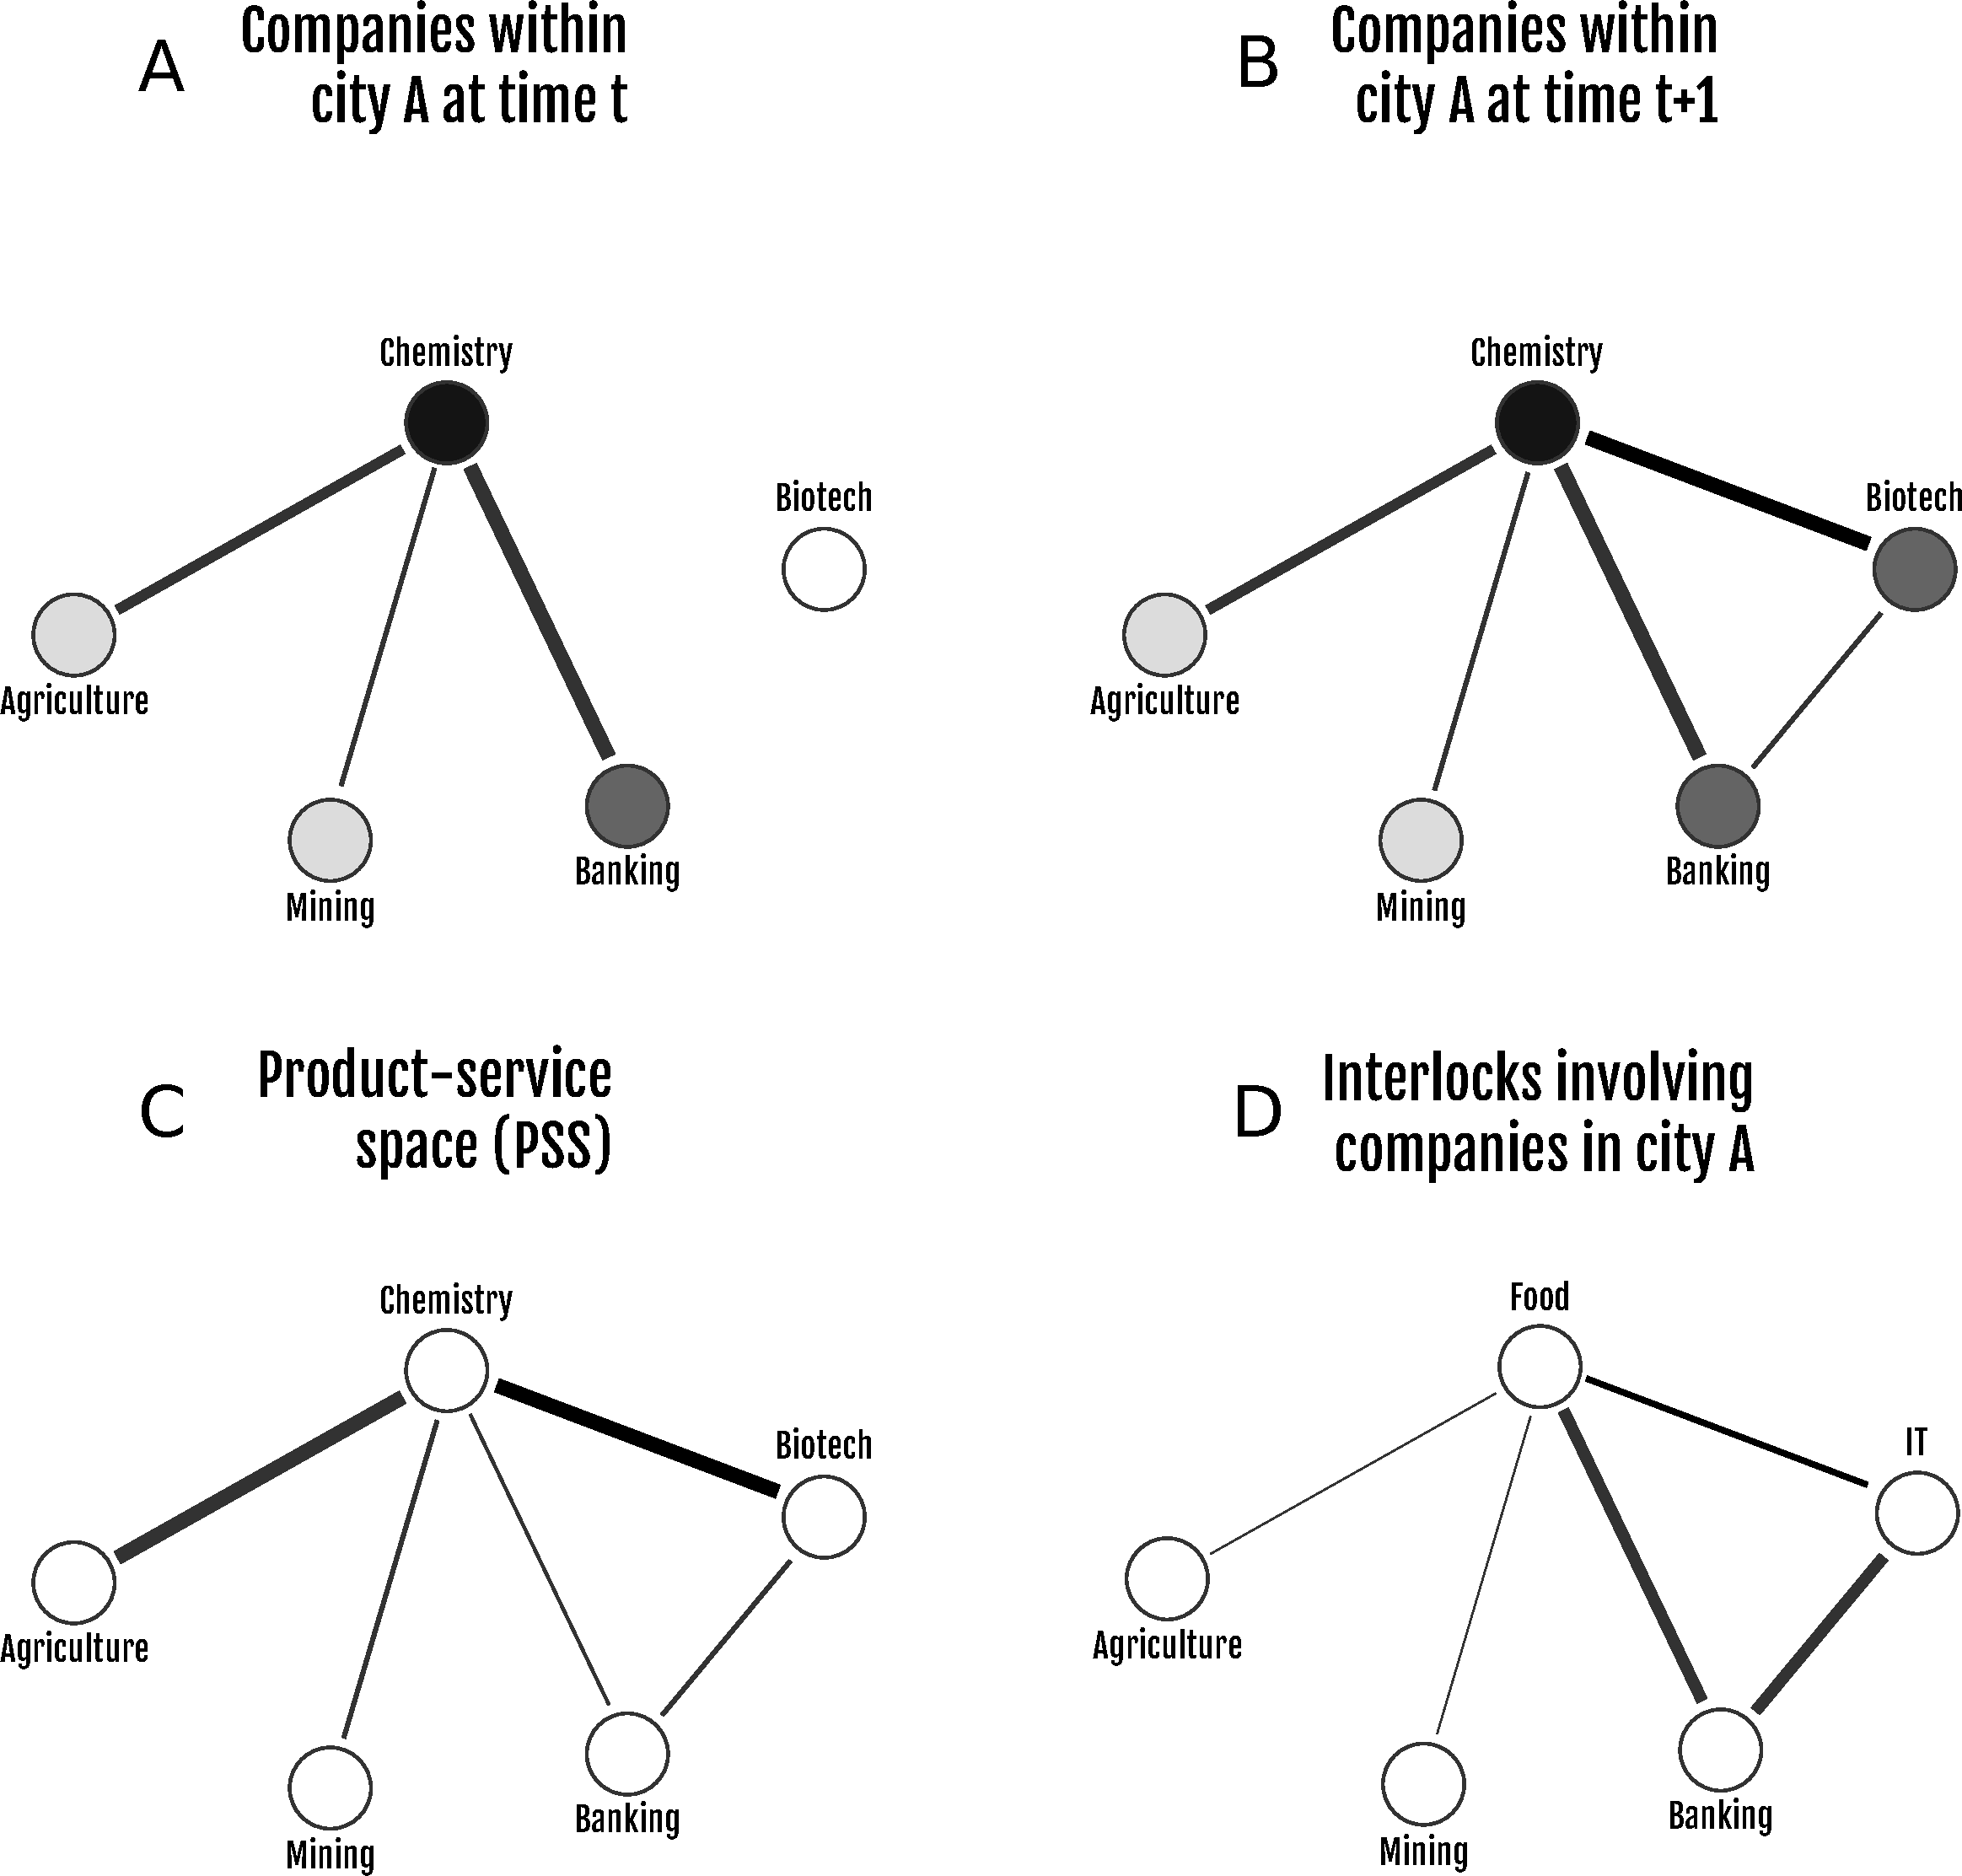
\includegraphics[width=.5\textwidth]{entropy.pdf}
\caption{.}
\label{fig:entropy}
\end{center}
\end{figure}

One method to study if interlocks are predictors of the diffusion process is conditional entropy $H(X|Y)$.
The conditional entropy  $H(Companies_{t_1}|Companies_{t_0})$ quantifies how much extra information we need to define the structure of the network at time 1 knowing the structure at time 0. 
If the network of interlocks between economic activities affect structural transformation we will find that $H(Companies_{t_1}|Companies_{t_0},Interlocks_{t_0}) < H(Companies_{t_1}|Companies_{t_0})$.
Other methods include using generative models such as ERGMs [ref] or SIENA [ref] to assess if the presence of interlocks at time $t$ is predicted by $Companies_{t_1}$
better than for $Companies_{t_0}$.
Such a models allow to control for node attributes (see below) and for recursive network effects 
-- e.g. the probability that there is an interlock A--C if there are interlocks A--B and B--C is increased (transitivity), and should be controlled.

There are several problems with this approach.
Firstly, we have explained that development creates interlocks (endogeneity problem).
The use of longitudinal data allows us to quantify the effect of interlocks on development,
independently of the effect of development on interlocks.
Secondly, there is a chance of self-selection bias.
Companies that want to develop a product in another sector may create interlocks with a company from economic activity beforehand.
However, if this is true, interlocks would also facilitate diffusion.
Finally, a most important bias is omitted variable bias.
If there is an underlying mechanism that produces the interlock at $time_1$ and the diffusion at $time_2$, 
we would find a false effect of interlocks on the diffusion process.
For example, cities that are developing fast (for whatever reason) may attract more interlocks than those who are not developing.
In order to investigate this possibility, we need to control for city economic indicators, such as infrastructure, resources, education, city size, population density and growth.
Other variables to control are sector size, country indicators and type of interlocks (within city versus between cities).
We can create random models using the product-service space and these variables to investigate their effect.
Importantly, this approach allows us not only to discover if interlocks play a role in the diffusive process, 
but also to unravel what other factors also play a role in it.
Moreover, positive effects of interlocks in the diffusive process would imply that companies should seek interlocks in companies that are adjacent in the product-service space.


\subsubsection{Interlocks affect the company space (at least) through innovation}
In section~\ref{sec:interlockspss}, we investigate if interlocks affect the diffusive process in the product-service space.
In this section, we hypothesize that the effect of interlocks in the diffusive process is caused at least partially by an improvement in collaboration and innovation.
Innovation has been linked to gaining competitive advantage~\citep{Hitt1996}, expanding market share ~\citep{Franko1989} and increasing firm performance~\citep{Morbey1988}.
Thus, a correlation in section~\ref{sec:pss} between the product-service space and innovation would not be surprising. 
The subquestion corresponding to this subsection is ``Do interlocks foster collaboration between companies and innovation?''.
In order to test this hypothesis we will use patent data.
Similarly to the interlock case, two companies are connected if they share a patent.
We can use generative models such as ERGMs or SIENA to assess if the presence of interlocks at time $t$ facilitates the presence of a shared patent at time $t+1$. 
Since we expect other factors to affect the probability of collaboration (such as the presence of a university in the city),
we would need to control for those factors (see ~\ref{sec:interlockspss}).


\subsection{Which factors affect interlocks}
\label{sec:factors}
The literature for the factors influencing interlock creation is more consistent.
Geographical distance, colonial history, language, education and social networks have been pointed as factors influencing the presence of interlocks [refs].
Time allowing, we will explore this idea at the micro-scale using generative models such as ERGMs [ref] or SIENA [ref].


\subsection{Other projects}
The data allow for the exploration of other projects, such as:
(i) Describe of the inequality among directors, studying if the inequality has its origin in the education.
(ii) Analyze the homogenization of coordinated and liberal market economies.
(iii) Quantify the independence of a given sector (e.g. food).
(iv) Measure the transference of power from domestic corporation to transnational corporations.
(v) Network motifs, which combination of interlocks between sectors are more likely than random.
(vi) (Lack of) independence of media or food sectors across regions,
(vii) Importance of the nation-state in economic networks